
\begin{questions}
\question{
Numerical solution
}
\begin{solution}
 If we are dealing with the jellium model, and a simple electron gas we can keep the density more or less constant
 \begin{equation}
   n(\vec{r}) = \frac{Ne}{\Omega},
 \end{equation}
and then our HF equations look like
\begin{equation}
  \begin{aligned}[b]
    & \left\{  -\frac{\hbar^2 \nabla^2}{2m} - \frac{Ne^2}{\Omega} \int_{(\Omega)} \frac{d^3r'}{|\vec{r} - \vec{r'}|} + 2\sum_{k'=occ} \int d^3 r' \frac{e^2}{|\vec{r} - \vec{r'}|} |\varphi_{\vec{k}'}|^2
    \right. \\
    & \left. - \sum_{k'=occ} \int \frac{e^2}{|\vec{r} - \vec{r'}|} \frac{\varphi^*_{\vec{k}'}(\vec{r}') \varphi_{\vec{k}}(\vec{r}') \varphi_{\vec{k}'}(\vec{r})}{\varphi_{\vec{k}}(\vec{r})} \right\} \varphi_{\vec{k}}(\vec{r})  = \varepsilon_{\vec{k}}^{HF} \varphi_{\vec{k}}(\vec{r}).
  \end{aligned}
\end{equation}
If we suppose our solutions are plane waves
\begin{equation}
  \varphi_{\vec{k}}(\vec{r}) = \frac{1}{\sqrt{\Omega}} e^{i\vec{k}\cdot \vec{r}},
\end{equation}
our equation modifies to
\begin{equation}
  \begin{aligned}[b]
    & \left\{  -\frac{\hbar^2 \nabla^2}{2m} - \frac{Ne^2}{\Omega} \int_{(\Omega)} \frac{d^3r'}{|\vec{r} - \vec{r'}|} + \frac{2}{\Omega} \sum_{k'=occ} \int d^3 r' \frac{e^2}{|\vec{r} - \vec{r'}|}
    \right. \\
    & \left. - \frac{1}{\Omega}\sum_{k'=occ} \int d^3\vec{r}'\frac{e^2}{|\vec{r} - \vec{r'}|} e^{i(\vec{k}' - \vec{k})\cdot(\vec{r}- \vec{r}')} \right\} e^{i\vec{k}\cdot \vec{r}}  = \varepsilon_{\vec{k}}^{HF} e^{i\vec{k}\cdot \vec{r}}.
  \end{aligned}
\end{equation}
Here we can notice that the second and third terms inside the curly brackets cancel each other
\begin{equation}
  - \frac{Ne^2}{\Omega} \int_{(\Omega)} \frac{d^3r'}{|\vec{r} - \vec{r'}|} + \frac{2e^2}{\Omega} \frac{N}{2} \int  \frac{d^3 r'}{|\vec{r} - \vec{r'}|} = 0,
\end{equation}
so, our problem now consists on knowing who the third therm is. We can see that the target term only depends on the distance $|\vec{r} - \vec{r'}|$, and therefore we can propose a variable change
\begin{equation}
  \int d^3\vec{r}' \frac{e^2}{|\vec{r} - \vec{r'}|} e^{i(\vec{k}' - \vec{k})\cdot(\vec{r}- \vec{r}')} = \int d^3z \frac{e^2}{z} e^{i(\vec{k}' - \vec{k})\cdot \vec{z}}.
\end{equation}
Now for the first term we can directly apply the kinetic energy operator and obtain
\begin{equation}
  -\frac{\hbar^2 \nabla^2}{2m}  e^{i\vec{k}\cdot \vec{r}} = \frac{\hbar^2 k^2}{2m}  e^{i\vec{k}\cdot \vec{r}},
\end{equation}
and as a consequence we will have
\begin{equation}
  \varepsilon_{\vec{k}}^{HF} = \frac{\hbar^2 k^2}{2m} - \frac{1}{\Omega}\sum_{k'=occ} \int d^3z \frac{e^2}{z} e^{i(\vec{k}' - \vec{k})\cdot \vec{z}},
\end{equation}
We are closer but not yet there, we need to analyze that second term and take it to a more friendly form.
Let's calculate further the term
\begin{equation}
  \varepsilon_{\vec{k}}^x = - \frac{1}{\Omega}\sum_{k'=occ} \int d^3z \frac{e^2}{z} e^{i(\vec{k}' - \vec{k})\cdot \vec{z}}.
\end{equation}
When we expand the Coulomb potential in Fourier series we will get
\begin{equation}
  \frac{e^2}{z} = \frac{1}{\Omega} \sum_{\vec{q}} e^{i\vec{q}\cdot \vec{z}} \frac{4\pi e^2}{q^2},
\end{equation}
using this in our equation yields
\begin{equation}
  \varepsilon_{\vec{k}}^x = - \frac{1}{\Omega^2}\sum_{k'=occ} \sum_{\vec{q}} e^{i\vec{q}\cdot \vec{z}} \frac{4\pi e^2}{q^2} \int d^3z  e^{i(\vec{q} -\vec{k}' + \vec{k})\cdot \vec{z}},
\end{equation}
but the term
\begin{equation}
  \int d^3z  e^{i(\vec{q} -\vec{k}' + \vec{k})\cdot \vec{z}} = \Omega \delta_{\vec{q} -\vec{k}' + \vec{k},0},
\end{equation}
therefore
\begin{equation}
  \varepsilon_{\vec{k}}^x = - \frac{1}{\Omega^2}\sum_{k'=occ} \frac{4\pi e^2}{|\vec{k}-\vec{k}'|^2} .
\end{equation}
We know how to turn the sums into integrals, so let's do that here
\begin{equation}
  \begin{aligned}[b]
    \varepsilon_{\vec{k}}^x &= - \frac{1}{(2\pi)^3}\int_{k'=occ} \frac{4\pi e^2}{|\vec{k}-\vec{k}'|^2}, \\
    & = - \frac{1}{(2\pi)^3}\int_{k'=0}^{k_F}dk' k'^2 \int_{\xi = -1}^1 d\xi \frac{4\pi e^2}{(k^2 + k'^2 - 2kk'\xi)^2}.
  \end{aligned}
\end{equation}
solving the integral we obtained the result we were looking for
\begin{equation}
  \varepsilon_{\vec{k}}^x = -\frac{e^2k_F}{2\pi} \left[ 2 + \frac{k_F^2 - k^2}{k\cdot k_F} \cdot \ln \left| \frac{k+k_F}{k-k_F} \right| \right].
\end{equation}
And finally we have the energy we were looking for
\begin{equation}
  \varepsilon_{\vec{k}}^{HF} = \frac{\hbar^2 k^2}{2m} - -\frac{e^2k_F}{2\pi} \left[ 2 + \frac{k_F^2 - k^2}{k\cdot k_F} \cdot \ln \left| \frac{k+k_F}{k-k_F} \right| \right]. \quad _\blacksquare
\end{equation}
From this we can derive the group velocity if we remember two things, first
\begin{equation}
  E = \hbar \omega,
\end{equation}
and
\begin{equation}
  v_g = \frac{d\omega}{dk}.
\end{equation}
Hence,
\begin{equation}
  \omega(k) = \frac{\hbar k^2}{2m} -\frac{e^2k_F}{\hbar 2\pi} \left[ 2 + \frac{k_F^2 - k^2}{k\cdot k_F} \cdot \ln \left| \frac{k+k_F}{k-k_F} \right| \right],
\end{equation}
and as a consequence
\begin{equation}
  \begin{aligned}[b]
    v_g &= \frac{\hbar k}{m} + \frac{e^2k_F}{\hbar 2\pi} \frac{(k^2 - k_F^2)^2 \ln((k + k_F)/(k - k_F)) - 2 k k_F (k^2 + k_F^2)}{k^2 k_F (k - k_F) (k + k_F)}, \\
    &= \frac{\hbar k}{m} + \frac{e^2}{2\hbar\pi} \frac{(k^2 - k_F^2)^2 \ln((k + k_F)/(k - k_F)) - 2 k k_F (k^2 + k_F^2)}{k^2 (k - k_F) (k + k_F)}.
  \end{aligned}
\end{equation}
Finally we can see this function ploted in fig. \ref{fig:enDisp}
\begin{center}
  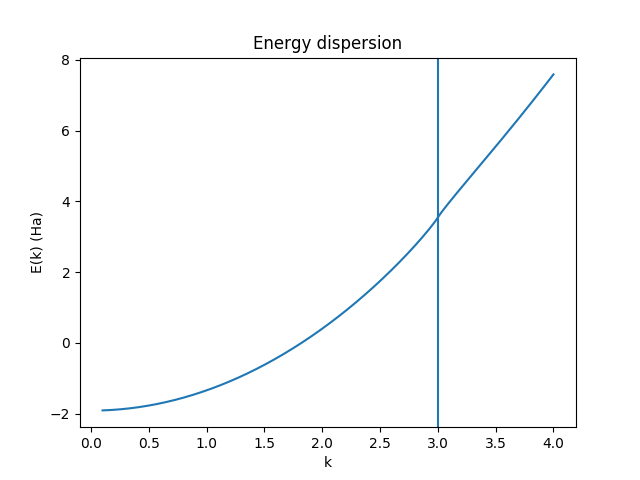
\includegraphics[width=110mm]{dispEn}
\end{center}

\captionof{figure}{Energy dispersion of a homogeneous gas, the vertical line corresponds to $k_F$.}\label{fig:enDisp}\vspace{0.5cm}

 \end{solution}

\end{questions}

%
% \begin{center}
%   \includegraphics[width=55mm]{}
% \end{center}
%
% \captionof{figure}{}\label{new}\vspace{0.5cm}
